\documentclass[border=6pt]{standalone}
\usepackage[T1]{fontenc}
\usepackage{mathptmx}
\usepackage{xcolor}
\usepackage{tikz}
\usetikzlibrary{positioning,arrows.meta,calc,shapes.geometric,decorations.pathmorphing}
\definecolor{lugar}{HTML}{CDE2FB}
\definecolor{atrator}{HTML}{F6C9B5}
\definecolor{tinta}{HTML}{3B3B38}
\definecolor{azul}{HTML}{2A78D6}
\definecolor{laranja}{HTML}{EB6834}
\definecolor{verde}{HTML}{1BAF7A}
\begin{document}
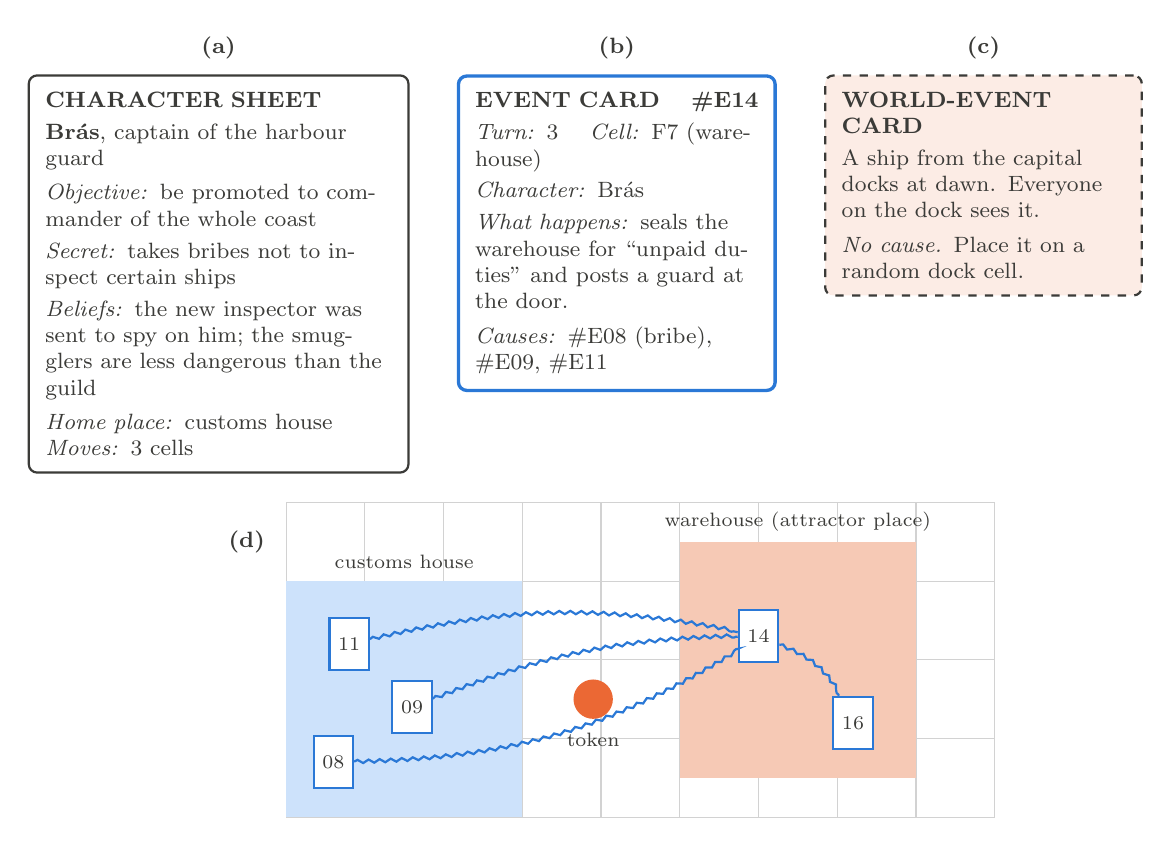
\begin{tikzpicture}[font=\footnotesize, every node/.style={text=tinta}]
  % --- ficha de personagem ---
  \node[draw=tinta, thick, rounded corners=3pt, fill=white, text width=4.4cm, inner sep=6pt, align=left] (ficha) at (0,0) {
    \textbf{CHARACTER SHEET}\\[2pt]
    \textbf{Brás}, captain of the harbour guard\\[3pt]
    \textit{Objective:} be promoted to commander of the whole coast\\[2pt]
    \textit{Secret:} takes bribes not to inspect certain ships\\[2pt]
    \textit{Beliefs:} the new inspector was sent to spy on him; the smugglers are less dangerous than the guild\\[3pt]
    \textit{Home place:} customs house\quad \textit{Moves:} 3 cells
  };
  \node[above=2pt of ficha.north, font=\footnotesize\bfseries] {(a)};

  % --- carta de evento ---
  \node[draw=azul, very thick, rounded corners=3pt, fill=white, text width=3.6cm, inner sep=6pt, align=left, anchor=north west] (carta) at ($(ficha.north east)+(0.6,0)$) {
    \textbf{EVENT CARD} \hfill \textbf{\#E14}\\[2pt]
    \textit{Turn:} 3 \quad \textit{Cell:} F7 (warehouse)\\[2pt]
    \textit{Character:} Brás\\[2pt]
    \textit{What happens:} seals the warehouse for ``unpaid duties'' and posts a guard at the door.\\[3pt]
    \textit{Causes:} \#E08 (bribe), \#E09, \#E11
  };
  \node[above=2pt of carta.north, font=\footnotesize\bfseries] {(b)};

  % --- carta de acontecimento do mundo ---
  \node[draw=tinta, thick, dashed, rounded corners=3pt, fill=atrator!35, text width=3.6cm, inner sep=6pt, align=left, anchor=north west] (mundo) at ($(carta.north east)+(0.6,0)$) {
    \textbf{WORLD-EVENT CARD}\\[2pt]
    A ship from the capital docks at dawn. Everyone on the dock sees it.\\[3pt]
    \textit{No cause.} Place it on a random dock cell.
  };
  \node[above=2pt of mundo.north, font=\footnotesize\bfseries] {(c)};

  % --- ficha + barbante (mini mesa) ---
  \begin{scope}[shift={($(carta.south)+(-4.2,-5.4)$)}]
    \foreach \x in {0,...,8} \foreach \y in {0,...,3} \draw[gray!35] (\x,\y) rectangle ++(1,1);
    \fill[lugar] (0,0) rectangle (3,3);
    \node[font=\scriptsize] at (1.5,3.25) {customs house};
    \fill[atrator] (5,0.5) rectangle (8,3.5);
    \node[font=\scriptsize] at (6.5,3.75) {warehouse (attractor place)};
    \foreach \x/\y/\n in {0.6/0.7/08, 1.6/1.4/09, 0.8/2.2/11, 6.0/2.3/14, 7.2/1.2/16}
      \node[draw=azul, thick, fill=white, minimum width=0.5cm, minimum height=0.66cm, inner sep=0pt, font=\scriptsize] (c\n) at (\x,\y) {\n};
    \draw[azul, thick, decorate, decoration={snake, amplitude=0.6pt, segment length=4pt}] (c08) to[bend right=15] (c14);
    \draw[azul, thick, decorate, decoration={snake, amplitude=0.6pt, segment length=4pt}] (c09) to[bend left=10] (c14);
    \draw[azul, thick, decorate, decoration={snake, amplitude=0.6pt, segment length=4pt}] (c11) to[bend left=12] (c14);
    \draw[azul, thick, decorate, decoration={snake, amplitude=0.6pt, segment length=4pt}] (c14) to[bend left=20] (c16);
    \fill[laranja] (3.9,1.5) circle (0.25);
    \node[font=\scriptsize, anchor=north] at (3.9,1.2) {token};
    \node[font=\footnotesize\bfseries] at (-0.5,3.5) {(d)};
  \end{scope}
\end{tikzpicture}
\end{document}
